% !TeX root = ../main.tex
% %%%%%%%%%%%%%%%%%%%%%%%%%%%%%%%%%%%%%%%%%%%%%%%%%%%%%%%%%%%%%%%%%%%%%%%%%%%%%%
% Monitoring
\chapter{Monitoring}
\label{chap:monitoring}

This chapter explains the whole process of monitoring, from compilation to error detection. First, the overall process of compilation is explained in \autoref{sec:runtimemonitoring}, then the generated file and some of its specifications are described in (\autoref{sec:generatedfile}).


% ------------------------------------------------------------------------------
% Runtime Monitoring
\section{Runtime Monitoring}
\label{sec:runtimemonitoring}

After writing all the desired robotic systems specifications, the file needs to be compiled to a monitoring Python module. This is currently done running the following script, from its location: \lstinline{python language.py properties.txt /home/ros_workspace/src/my_pkg/src}.

The \textit{language.py} file needs to be run as a Python file and takes as arguments:

\begin{enumerate}
    \item The specifications file;
    \item The path where the the generated Python monitoring module will be generated.
\end{enumerate}

The given directory for the generated file should be under a ROS workspace for the compilation to succeed. This is because, during the compilation, access to information like the available ROS messages might be necessary.

The monitoring file can now run as an independent ROS node, integrated into a launch file, or using \textit{rosrun} in the console to execute it.


% ------------------------------------------------------------------------------
% Generated File
\section{Compilation} 
\label{sec:generatedfile}

\todo{explain sections}

This section *then the generated file and some of its specifications are described*

% ------------------------------------------------------------------------------
% Runtime Monitoring
\subsection{Architecture}
\label{ssec:compileArchitecture}

\todo{Diagram/Figure here somewhere and see whole subsection}

The node executes a loop at a delineated rate, doing the following tasks:

\begin{enumerate}
    \item Check if the defined simulation timeout time has reached.
    \item Save the current simulation state.
    \item Verify the properties using the saved states and calling each created function. An independent function with the necessary computations for verifying the property is defined for each base property.
\end{enumerate}


\todo{Maybe add section here about type checking?}

% ------------------------------------------------------------------------------
% Runtime Monitoring
\subsection{Code Generation}
\label{ssec:compileCtx}

In order to generate the monitoring code some context is saved when parsing through the abstract syntax tree created from the specification file.

The saved context is essentialy separated in five lists: \nameref{sssec:compileModels}, \nameref{sssec:compileAssoc}, \nameref{sssec:compileVars}, \nameref{sssec:compileSubs}, and \nameref{sssec:compileProp}.

The information saved in these data structures will aftwards be used in translation rules between the source code to create the generated code.

\todo{translation rules between the source code and the generated code. Of all}


% ------------------------------------------------------------------------------
% Runtime Monitoring
\subsubsection{Models}
\label{sssec:compileModels}

The data structure of each model saved in the context is composed of:

\begin{enumerate}
    \item The name during execution of the object in the simulation that is being modeled.
    \item The correspondent function the model refers to, for example \textit{velocity} or \textit{distance}.
    \item The Message type of the data structure of the \textit{topic} to subscribe.
\end{enumerate}

For each entry in the \textit{Model} of an object: A model data structure will be saved in the context. And a subscriber data structure will be created that will subscribe to the correspondent \textit{topic} of the modeled object.

The subscriber and variable in the generated code associated to each entry will have a unique name composed of the object name plus the function associated in that entry.


% ------------------------------------------------------------------------------
% Runtime Monitoring
\subsubsection{Associations}
\label{sssec:compileAssoc}

The data structure of each association saved in the context is composed of:

\begin{enumerate}
    \item The name of the association in the specification.
    \item The name of the variable associated with the association.
\end{enumerate}

When specifying an association a new variable data structure is created in the context. The new variable has the prefix of an association aswell as its name. In the generated code the new variable will point to the variable created in the right side of the association.


% ------------------------------------------------------------------------------
% Runtime Monitoring
\subsubsection{Variables}
\label{sssec:compileVars}

The data structure of each variable saved in the context is composed of:

\begin{enumerate}
    \item Variable name in the specification.
    \item Variable name to use in generated code.
\end{enumerate}

The variables names to be used in the generated code will have different sufixes and prefixes depending on: Their types, if they originate from a model, declaration, function or association. In this way it is easier to identify variable relations during the compilation of the generated code.

All simulation primitives are hardcoded to get their absolute value from the simulator \textit{topic}.
To retrieve the correct string for each primitive to be used in the generated code, an auxiliar function \textit{sim\_funcs} was created:

\begin{lstlisting}[language=Python]
    def sim_funcs(object_, func, args, ctx):
    """Add var to the context and return var name for the output file (Considering the function used)"""
    var_name, extract = None, None
    if func == "position":
        args = ["position"] + args
        var_name = object_ + "_" + "_".join(args) + "_var_sim"
        extract = (
            "model_states_msg.pose[model_states_indexes['"
            + object_
            + "']]."
            + ".".join(args)
        )
    elif func == "velocity":
        var_name = object_ + "_velocity_" + "_".join(args) + "_var_sim"
        if args == []:
            extract = (
                "((model_states_msg.twist[model_states_indexes['"
                + object_
                + "']].linear.x)**2 + (model_states_msg.twist[model_states_indexes['"
                + object_
                + "']].linear.y)**2 + (model_states_msg.twist[model_states_indexes['"
                + object_
                + "']].linear.z)**2"
                + ")**(0.5)"
            )
        else:
            extract = (
                "model_states_msg.twist[model_states_indexes['"
                + object_
                + "']]."
                + ".".join(args)
            )
    elif func == "localization_error":
        var_name = object_ + "_localization_error"
        args = ctx.model_msgtype(object_, "position")
        extract = (
            "((model_states_msg.pose[model_states_indexes['"
            + object_
            + "']].position.x - "
            + object_
            + "_position_msg."
            + args
            + ".x)**2 + (model_states_msg.pose[model_states_indexes['"
            + object_
            + "']].position.y - "
            + object_
            + "_position_msg."
            + args
            + ".y)**2 + (model_states_msg.pose[model_states_indexes['"
            + object_
            + "']].position.z - "
            + object_
            + "_position_msg."
            + args
            + ".z)**2)**(0.5)"
        )
    elif func == "distanceZ":
        object2 = args[0]
        var_name = object_ + "_" + object2 + "_distanceZ"
        extract = (
            "((model_states_msg.pose[model_states_indexes['"
            + object_
            + "']].position.x - model_states_msg.pose[model_states_indexes['"
            + object2
            + "']].position.x)**2 + (model_states_msg.pose[model_states_indexes['"
            + object_
            + "']].position.y -"
            + "model_states_msg.pose[model_states_indexes['"
            + object2
            + "']].position.y)**2 + (model_states_msg.pose[model_states_indexes['"
            + object_
            + "']].position.z - model_states_msg.pose[model_states_indexes['"
            + object2
            + "']].position.z)**2)**(0.5)"
        )
    elif func == "distance":
        object2 = args[0]
        var_name = object_ + "_" + object2 + "_distance"
        extract = (
            "((model_states_msg.pose[model_states_indexes['"
            + object_
            + "']].position.x - model_states_msg.pose[model_states_indexes['"
            + object2
            + "']].position.x)**2 + (model_states_msg.pose[model_states_indexes['"
            + object_
            + "']].position.y -"
            + "model_states_msg.pose[model_states_indexes['"
            + object2
            + "']].position.y)**2)**(0.5)"
        )
    ctx.add_var(var_name, extract)
    return "states[0]['" + var_name + "']"
\end{lstlisting}


% ------------------------------------------------------------------------------
% Runtime Monitoring
\subsubsection{Subscribers}
\label{sssec:compileSubs}

The data structure of each subscriber saved in the context is composed of:

\begin{enumerate}
    \item The Topic name which to subscribe.
    \item The Message type associated with the topic.
    \item The Library from which the Message type originates
    \item The Subscriber name in the generated code
\end{enumerate}

A subscriber relates in the specification to a \textit{declaration}, a \textit{model} entry, or the default simulator information \textit{topic}.

The Library is necessary in order to make an import of the Message type in the generated code. The Library is obtained through a python subsprocess:

\begin{lstlisting}[language=Python]
    command = f"cd {self.filepath} | rosmsg show {msg_type}"
\end{lstlisting}

The generated monitoring file declares the needed subscribers and uses ApproximateTimeSynchronizer to call the callback function. The ApproximateTimeSynchronizer synchronizes messages by their timestamp and if they do not have a header, uses the ROS time.


% ------------------------------------------------------------------------------
% Runtime Monitoring
\subsubsection{Properties}
\label{sssec:compileProp}

\todo{all here}

The data structure of each property saved in the context is composed of:

\begin{enumerate}
    \item Line in the specification file.
    \item the type of property.
    \item built string array with the necessary comparisons to build a boolean assertion about the property in the generated code.
\end{enumerate}


% ------------------------------------------------------------------------------
% Runtime Monitoring
\subsection{State}
\label{ssec:compileState}

\todo{translation rules between the source code and the generated code. Of all}

A callback function is called every time a new message from one of the subscribers is received. The callback function saves the relevant information for property checking in a global variable. This information serves as a current "screenshot" of the simulation representing its current state.

obtained by the callback function. This is necessary because the callback function is called at fluctuating rates, and the objective is to save multiple "screenshots" of the simulation at the loop fixed rate to make correlations with past states.


% ------------------------------------------------------------------------------
% Error Messages
\subsection{Error Messages}
\label{ssec:errormessages}

An error message starts by stating the line in the specification file which resulted in an error as well as showing the property where the error originated.

Afterward, I use the current saved state of the simulation to show the values at the time of failure of all the variables present in the property that originated the error.

\begin{figure}[htb]
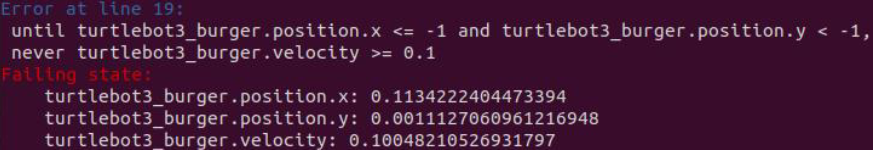
\includegraphics[width=\textwidth]{images/error_message1.png}
\caption{Example of an error message.} \label{fig:monerror}
\end{figure}